%% ============================================================
% f2012_shandong_sci_q18_solid.tex
%% 2012 山东卷（理科）第 18 题 几何体：等腰梯形 ABCD 为底，FC⊥平面 ABCD
%% 来源 PDF：普通高考/2012/2012山东理.pdf 第 2 页（印面 760）第 1 栏
%% 坐标取自原页矢量层（bp），原点为图区左上角 (240.0,138.0)，y 向下；虚线照原页。
%% ============================================================
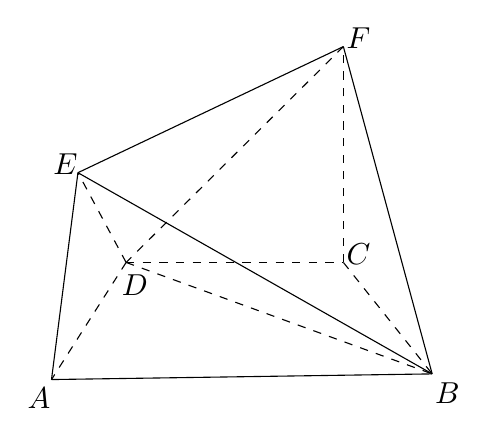
\begin{tikzpicture}[x=1bp,y=-1bp,
  every node/.style={inner sep=0,font=\fontsize{10.5pt}{12.6pt}\selectfont},
  line cap=butt, line join=miter]
  \draw[line width=0.3985bp] (24.035,50.133) -- (119.594,4.738);
  \draw[line width=0.3985bp] (24.035,50.133) -- (14.516,124.605);
  \draw[line width=0.3985bp] (151.559,122.566) -- (119.594,4.738);
  \draw[line width=0.3985bp] (151.559,122.566) -- (14.516,124.605);
  \draw[line width=0.3985bp] (24.035,50.133) -- (151.559,122.566);
  \draw[line width=0.3985bp, dash pattern=on 2.989bp off 2.989bp] (41.379,82.441) -- (24.035,50.133);
  \draw[line width=0.3985bp, dash pattern=on 2.989bp off 2.989bp] (41.379,82.441) -- (119.594,82.441);
  \draw[line width=0.3985bp, dash pattern=on 2.989bp off 2.989bp] (41.379,82.441) -- (14.516,124.605);
  \draw[line width=0.3985bp, dash pattern=on 2.989bp off 2.989bp] (41.379,82.441) -- (151.559,122.566);
  \draw[line width=0.3985bp, dash pattern=on 2.989bp off 2.989bp] (119.594,82.441) -- (119.594,4.738);
  \draw[line width=0.3985bp, dash pattern=on 2.989bp off 2.989bp] (119.594,4.738) -- (41.379,82.441);
  \draw[line width=0.3985bp, dash pattern=on 2.989bp off 2.989bp] (119.594,82.441) -- (151.559,122.566);
  \node[anchor=base west] at (120.56,5.38) {$F$};
  \node[anchor=base west] at (15.03,50.79) {$E$};
  \node[anchor=base west] at (120.53,83.11) {$C$};
  \node[anchor=base west] at (39.66,94.49) {$D$};
  \node[anchor=base west] at (152.39,133.12) {$B$};
  \node[anchor=base west] at (5.74,135.16) {$A$};
\end{tikzpicture}
